%
% LaTeX report template 
%

% This is a comment: in LaTeX everything that in a line comes
% after a "%" symbol is treated as comment

\documentclass[11pt, a4paper]{article}
\usepackage{graphicx}
\usepackage{amsmath}
\usepackage{listings}
\usepackage{url}
\usepackage{float}
\usepackage{xcolor}

\definecolor{codegreen}{rgb}{0,0.6,0}
\definecolor{codegray}{rgb}{0.5,0.5,0.5}
\definecolor{codepurple}{rgb}{0.58,0,0.82}
\definecolor{backcolour}{rgb}{0.95,0.95,0.92}

\lstdefinestyle{mystyle}{
    backgroundcolor=\color{backcolour},   
    commentstyle=\color{codegreen},
    keywordstyle=\color{magenta},
    numberstyle=\tiny\color{codegray},
    stringstyle=\color{codepurple},
    basicstyle=\ttfamily\footnotesize,
    breakatwhitespace=false,         
    breaklines=true,                 
    captionpos=b,                    
    keepspaces=true,                 
    numbers=left,                    
    numbersep=5pt,                  
    showspaces=false,                
    showstringspaces=false,
    showtabs=false,                  
    tabsize=2
}

\lstset{style=mystyle}

\title{EE2703: Applied Programming Lab \\ Assignment No 4: Fourier Approximations} % Title

\author{Ishaan Agarwal \\ EE20B046} % Author name

\date{\today} % Date for the report
\begin{document}		
		
\maketitle % Insert the title, author and date

\section{Introduction}
%Create new section;it is autonumbered
In this assignment, we try to fit the two functions $\exp(x)$ and $\cos(\cos(x))$ using the Fourier series.

\[a_0 + \sum_{n=1}^{\infty} [a_n\cos(nx) + b_n\cos(nx)] \]

where the coefficients $a_n$ and $b_n$ are given by:

\[ a_0 = \frac{1}{2\pi} \int_{0}^{2\pi} f(x) \,dx \]

\[ a_n = \frac{1}{\pi} \int_{0}^{2\pi} f(x)cos(nx) \,dx \]

\[ b_n = \frac{1}{\pi} \int_{0}^{2\pi} f(x)sin(nx) \,dx \]
\section{Questions}
\subsection{Question 1: Defining and Plotting the functions}
To define the Python functions for the two functions above that take a vector or scalar input and return corresponding vector or scalar output, this is accomplished using \texttt{np.exp()} and \texttt{np.cos(np.cos())} \\
These functions are then plotted over the interval $[-2\pi, 4\pi]$, $\cos(\cos(x))$ is periodic with period $\pi$ and thus we don't need a periodic extension, whereas $\exp(x)$ is aperiodic and thus we need to create a periodic extension of it from $[0, 2\pi]$\\

\begin{lstlisting}[language = Python]
#defining exponential function
def exp(x):
    return np.exp(x)

#defining cos(cos(x)) function
def cos_cos(x):
    return np.cos(np.cos(x))

#plotting the functions over (-2*pi, 4*pi)
x = np.linspace(-2*np.pi, 4*np.pi, 600)
x1 = np.linspace(-2*np.pi, 0, 200)
x2 = np.linspace(0, 2*np.pi, 200)
x3 = np.linspace(2*np.pi, 4*np.pi, 200)
y_true = exp(x)
y = np.zeros(len(x))
y[0:200] = exp(x2)
y[200:400] = exp(x2)
y[400:600] = exp(x2)
z = cos_cos(x)

plt.semilogy(x, y_true, label='True Value of exp(x)', color='red')
plt.semilogy(x, y, label='Periodic extended Value of exp(x)', color='blue')
plt.xlabel('x')
plt.ylabel('y')
plt.title('Plot of exp(x)')
plt.legend()
plt.grid()
plt.show()

plt.plot(x, z, label='cos(cos(x))')
plt.xlabel('x')
plt.ylabel('z')
plt.title('Plot of cos(cos(x))')
plt.legend()
plt.grid()
plt.show()
\end{lstlisting}

\begin{figure}[H]
     \centering
     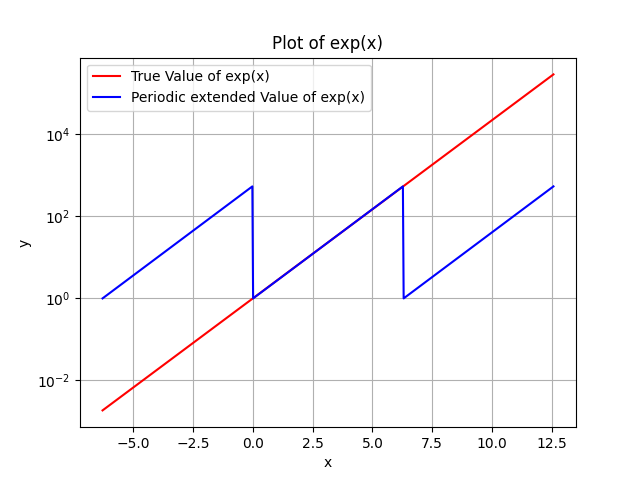
\includegraphics[scale=0.8]{Figure_1.png}
\end{figure}

\begin{figure}[H]
     \centering
     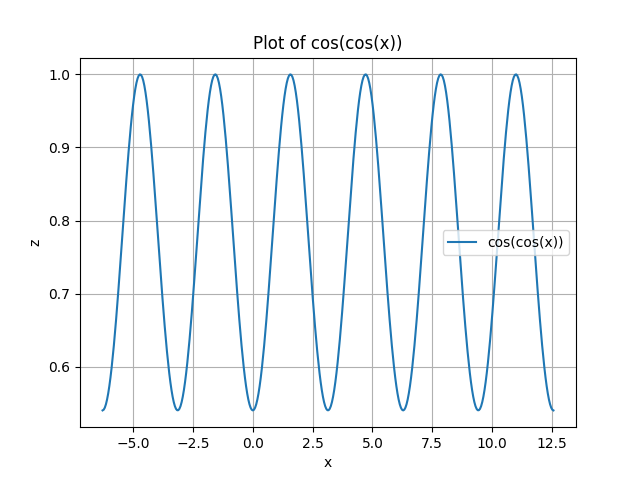
\includegraphics[scale=0.8]{Figure_2.png}
\end{figure}





\subsection{Question 2: Obtaining the fourier coefficients}
Here, we try to obtain the first 51 fourier series coefficients $a_0, a_1, ... a_{25}, b_0, b_1, ...b_{25}$. \\
So, we create a dictionary mapping the two functions, we also create two new functions to be integrated namely, $u(x, k, func)$ and $v(x, k, func)$. Then, we use \texttt{scipy.integrate.quad} and pass the additional arguments namely $k$ and $func$ using the parameter \texttt{args}. In this way, we have defined functions to compute Fourier series coefficients. \\

\begin{lstlisting}[language = Python]
#dictionary mapping the two functions exp(x) and cos(cos(x))
dict = {'exp(x)':exp, 'cos(cos(x))':cos_cos}


#defining u(x, k) and v(x, k) functions for exp(x)
def u(x, k, func):
    return dict[func](x)*np.cos(k*x)
def v(x, k, func):
    return dict[func](x)*np.sin(k*x)


#calculating fourier coefficients for exp(x)
def a(k, func):
    return integrate.quad(u, 0, 2*np.pi, args = (k, func))[0]/(np.pi)

def b(k, func):
    return integrate.quad(v, 0, 2*np.pi, args = (k, func))[0]/(np.pi)

def a0(func):
    return integrate.quad(u, 0, 2*np.pi, args = (0, func))[0]/(2*np.pi)
\end{lstlisting}


\subsection{Question 3: Plotting the coefficients}
We use a for loop to calculate the required coefficients using our earlier created functions and store them in numpy arrays. We now plot the coefficients, once on a semilogy scale and then on a loglog scale for both the functions. \\

\begin{lstlisting}[language = Python]
#storing all coefficients of exp(x) in one list
coeff_exp = []
coeff_exp.append(a0('exp(x)'))
for k in range(1, 26):
    coeff_exp.append(a(k, 'exp(x)'))
    coeff_exp.append(b(k, 'exp(x)'))

#storing all coefficients of cos(cos(x)) in one list
coeff_coscos = []
coeff_coscos.append(a0('cos(cos(x))'))
for k in range(1, 26):
    coeff_coscos.append(a(k, 'cos(cos(x))'))
    coeff_coscos.append(b(k, 'cos(cos(x))'))

#plotting the coefficients vs n for exp(x)
plt.semilogy(range(51), np.abs(coeff_exp), 'ro', label='coefficients for exp(x)')
plt.title('Semilog Plot of coefficients vs n for exp(x)')
plt.xlabel('n')
plt.ylabel('coefficients')
plt.legend()
plt.grid()
plt.show()

plt.loglog(range(51), np.abs(coeff_exp), 'ro', label='coefficients for exp(x)')
plt.title('Loglog Plot of coefficients vs n for exp(x)')
plt.xlabel('n')
plt.ylabel('coefficients')
plt.legend()
plt.grid()
plt.show()

#plotting the coefficients vs n for cos(cos(x))
plt.semilogy(range(51), np.abs(coeff_coscos), 'ro', label='coefficients for cos(cos(x))')
plt.title('Semilogy Plot of coefficients vs n for cos(cos(x))')
plt.xlabel('n')
plt.ylabel('coefficients')
plt.legend()
plt.grid()
plt.show()

plt.loglog(range(51), np.abs(coeff_coscos), 'ro', label='coefficients for cos(cos(x))')
plt.title('Loglog Plot of coefficients vs n for cos(cos(x))')
plt.xlabel('n')
plt.ylabel('coefficients')
plt.legend()
plt.grid()
plt.show()

\end{lstlisting}

\begin{figure}[H]
     \centering
     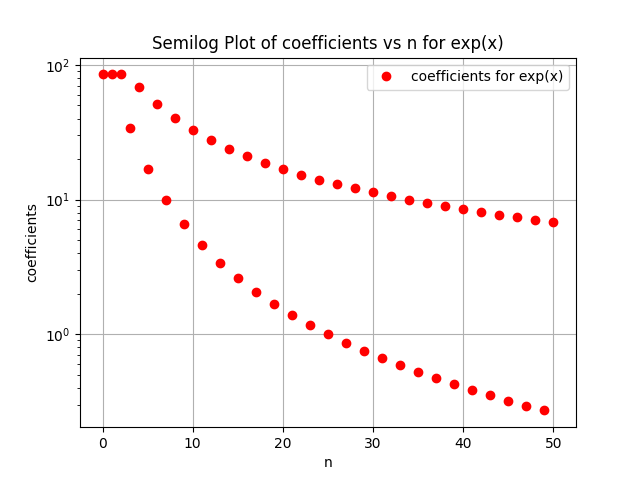
\includegraphics[scale=0.8]{Figure_3.png}
\end{figure}

\begin{figure}[H]
     \centering
     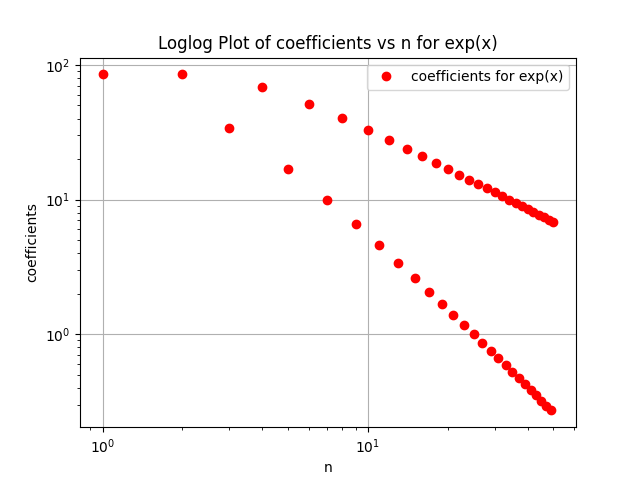
\includegraphics[scale=0.8]{Figure_4.png}
\end{figure}

\begin{figure}[H]
     \centering
     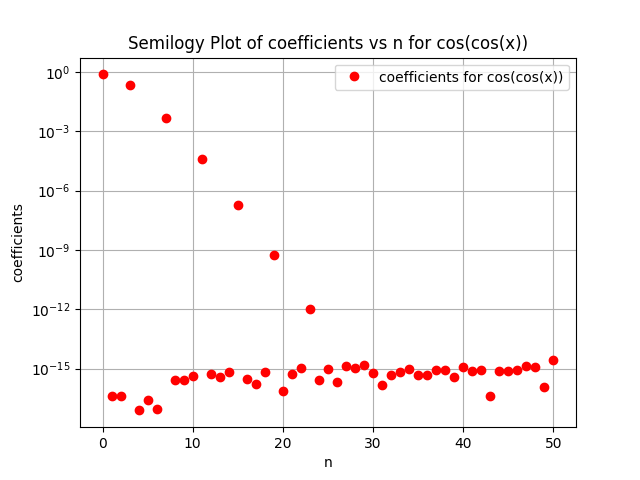
\includegraphics[scale=0.8]{Figure_5.png}
\end{figure}


\begin{figure}[H]
     \centering
     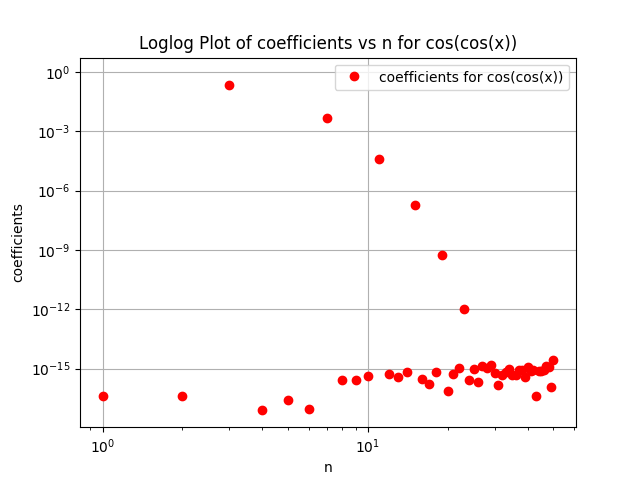
\includegraphics[scale=0.8]{Figure_6.png}
\end{figure}


\begin{itemize}
\item Here, we notice that the $b_n$ coefficients in the second case are nearly zero. This is because the function $\cos(\cos(x))$ is even and thus the odd sinusoid frequencies must not exist. 
\item We also notice that the decay for the coefficients is quick, this is because the frequency of $\cos(\cos(x))$ is relatively low, $=\frac{1}{\pi}$ and thus the contribution of the higher sinusoids is very low. 
\item On solving, we see that the magnitude of the coefficients of $\exp(x)$ varies with $n$ as $\frac{1}{n^2+1}$. Thus, for large n, $\log(a_n)$ and $log(b_n)$ vary approximately as $-2\log(n)$. Thus, the loglog plot becomes approximately linear for large n. Similarly, the coefficients of $\cos(\cos(x))$ would be approximately exponential with n. Thus, the semilog plot is linear.
\end{itemize}




\subsection{Question 4 and 5: The least squares Approach}
We notice that our earlier approach, even though is exactly right, is computationally expensive since we're calculating multiple integrals to get the coefficients. An approximate, but computationally efficient way to solve the problem is to convert this into a matrix problem and then use the least squares approach to solve it. \\
The Matrix equation is:
\[
\begin{bmatrix}
1 & \cos(x_1) & \sin(x_1) & ... & \cos(25x_1) & \sin(25x_1)\\
1 & \cos(x_2) & \sin(x_2) & ... & \cos(25x_2) & \sin(25x_2)\\
... & ... & ... & ... & ... & ...\\
1 & \cos(x_{400}) & \sin(x_{400}) & ... & \cos(25x_{400}) & \sin(25x_{400})
\end{bmatrix}
\begin{bmatrix}
a_0\\
a_1\\
b_1\\
a_2\\
b_2\\
...\\
a_{25}\\
b_{25}
\end{bmatrix}=
\begin{bmatrix}
f(x_1)\\
f(x_2)\\
f(x_3)\\
...\\
f(x_{400})
\end{bmatrix}
\]

This can be written as $Ac = b$
Thus, the coefficient matrix $c$ is obtained by minimising the square error using \texttt{np.linalg.lstsq()}.

\begin{lstlisting}[language = Python]
#using least squares method to calculate fourier coefficients

x = np.linspace(0, 2*np.pi, 401)
x = x[:-1] #drop last element to have proper periodic integral

b1 = exp(x)
A = np.zeros((400, 51))
A[:,0] = 1
for k in range(1, 26):
    A[:, 2*k-1] = np.cos(k*x)
    A[:, 2*k] = np.sin(k*x)
#finding the least squares solution c1
c1 = np.linalg.lstsq(A, b1)[0] #best fit vector

b2 = cos_cos(x)
A = np.zeros((400, 51))
A[:,0] = 1
for k in range(1, 26):
    A[:, 2*k-1] = np.cos(k*x)
    A[:, 2*k] = np.sin(k*x)
#finding the least squares solution c2
c2 = np.linalg.lstsq(A, b2)[0] #best fit vector

#plotting the new obtained coefficients along with the true values
plt.semilogy(range(51), np.abs(c1), 'ro', label='Estimated coefficients for exp(x)', alpha = 0.5)
plt.semilogy(range(51), np.abs(coeff_exp), 'go', label='True coefficients for exp(x))', alpha = 0.5)
plt.title('Semilog Plot of estimated coefficients and true coefficients vs n for exp(x)')
plt.xlabel('n')
plt.ylabel('Coefficients')
plt.legend()
plt.grid()
plt.show()

plt.loglog(range(51), np.abs(c1), 'ro', label='Estimated coefficients for exp(x)', alpha = 0.5)
plt.loglog(range(51), np.abs(coeff_exp), 'go', label='True coefficients for exp(x),', alpha = 0.5)
plt.title('Loglog Plot of estimated coefficients and true coefficients vs n for exp(x)')
plt.xlabel('n')
plt.ylabel('Coefficients')
plt.legend()
plt.grid()
plt.show()

plt.semilogy(range(51), np.abs(c2), 'ro', label='Estimated coefficients for cos(cos(x))', alpha = 0.5)
plt.semilogy(range(51), np.abs(coeff_coscos), 'go', label='True coefficients for cos(cos(x))', alpha = 0.5)
plt.title('Semilog Plot of estimated coefficients and true coefficients vs n for cos(cos(x))')
plt.xlabel('n')
plt.ylabel('Coefficients')
plt.legend()
plt.grid()
plt.show()

plt.loglog(range(51), np.abs(c2), 'ro', label='Estimated coefficients for cos(cos(x))', alpha = 0.5)
plt.loglog(range(51), np.abs(coeff_coscos), 'go', label='True coefficients for cos(cos(x))', alpha = 0.5)
plt.title('Loglog Plot of estimated coefficients and true coefficients vs n for cos(cos(x))')
plt.xlabel('n')
plt.ylabel('Coefficients')
plt.legend()
plt.grid()
plt.show()


\end{lstlisting}

The corresponding plots are:

\begin{figure}[H]
     \centering
     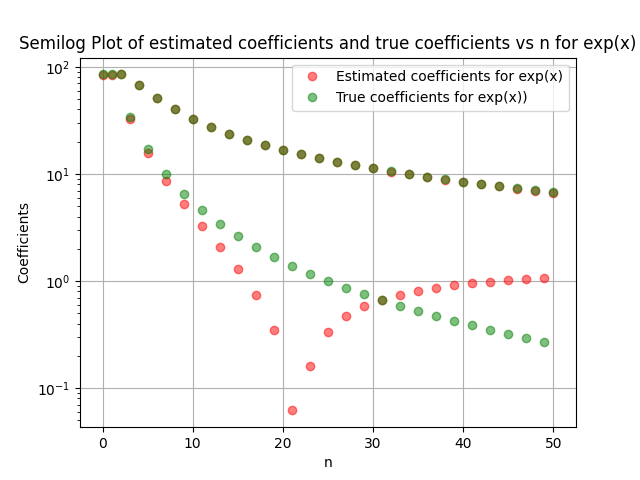
\includegraphics[scale=0.8]{Figure_7.png}
\end{figure}

\begin{figure}[H]
     \centering
     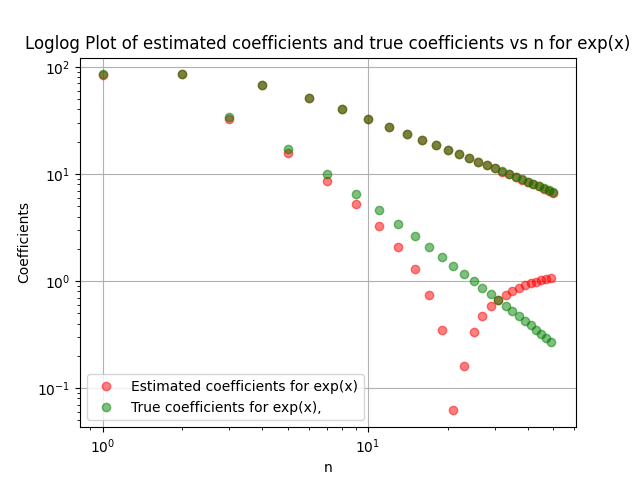
\includegraphics[scale=0.8]{Figure_8.png}
\end{figure}


\begin{figure}[H]
     \centering
     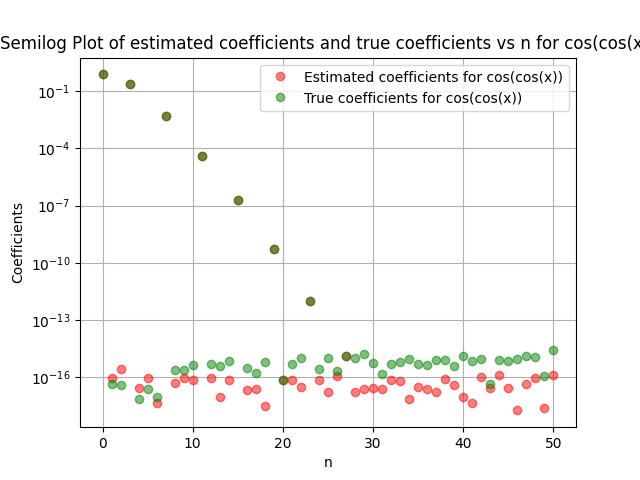
\includegraphics[scale=0.8]{Figure_9.png}
\end{figure}


\begin{figure}[H]
     \centering
     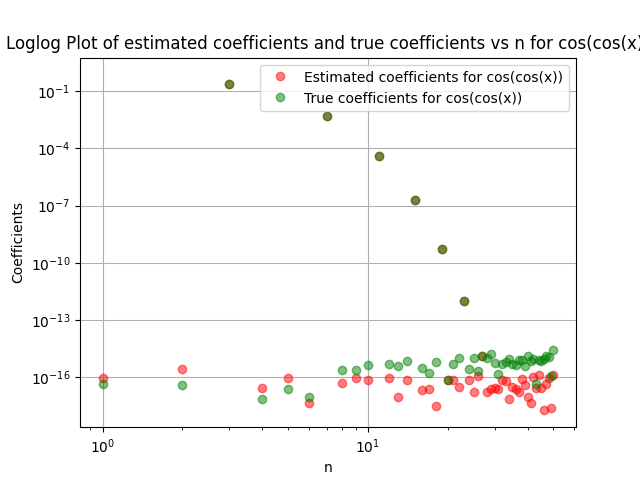
\includegraphics[scale=0.8]{Figure_10.png}
\end{figure}


Here, we notice that the approximate coefficients for the $\cos(\cos(x))$ plot are much closer to the true values than for $\exp(x)$ plot. This is because the former is periodic with period $\pi$ and thus the fourier series approximation is very close to the true value whereas this is not the case for the latter.

\subsection{Question 6: Analysing the error between estimated and true values}
We now find the error and maximum error in the obtained coefficients using least squares approach and try to plot it. \\

\begin{lstlisting}[language = Python]
#finding the absolute error between estimated and true value of fourier coefficients
error_exp = np.absolute(c1 - coeff_exp)
error_coscos = np.absolute(c2 - coeff_coscos)

#find the maximum error
max_error_exp = np.max(error_exp)
max_error_coscos = np.max(error_coscos)

#plotting the error
plt.plot(range(51), error_exp, 'ro', label='Error for exp(x)')
plt.title('Plot of error vs n for exp(x)')
plt.xlabel('n')
plt.ylabel('Error')
plt.legend()
plt.grid()
plt.show()

plt.plot(range(51), error_coscos, 'ro', label='Error for cos(cos(x))')
plt.title('Plot of error vs n for cos(cos(x))')
plt.xlabel('n')
plt.ylabel('Error')
plt.legend()
plt.grid()
plt.show()
\end{lstlisting}

\begin{figure}[H]
     \centering
     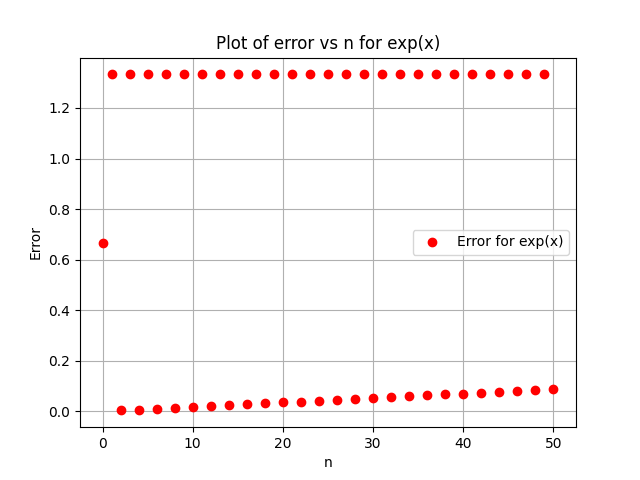
\includegraphics[scale=0.8]{Figure_11.png}
\end{figure}

\begin{figure}[H]
     \centering
     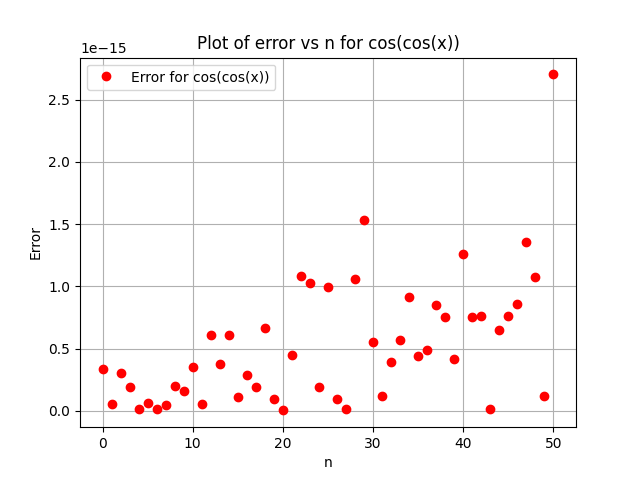
\includegraphics[scale=0.8]{Figure_12.png}
\end{figure}


The maximum error obtained is:\\
for $\exp(x)$: 1.33\\
for $\cos(\cos(x))$: $2.70 * 10^{-15}$
\\
which is in accordance with our earlier understanding.


\subsection{Question 7: Plotting estimated functions}
Here, we try to obtain plots of our functions using the approximate coefficients calculated using the least squares approach, the matrix product $M = Ac$ gives the function values. \\

\begin{lstlisting}[language = Python]
#Plotting the estimated functions A*c1 and A*c2
b1_est = np.dot(A, c1)
b2_est = np.dot(A, c2)

plt.semilogy(x, b1_est, 'go', label='Estimated function for exp(x)', alpha = 0.5)
plt.semilogy(x, b1, 'k', label='True Value')
plt.title('Plot of estimated function vs x for exp(x)')
plt.xlabel('x')
plt.ylabel('y')
plt.legend()
plt.grid()
plt.show()

plt.plot(x, b2_est, 'go', label='Estimated function for cos(cos(x))', alpha = 0.5)
plt.plot(x, b2, 'k', label='True Value')
plt.title('Plot of estimated function vs x for cos(cos(x))')
plt.xlabel('x')
plt.ylabel('y')
plt.legend()
plt.grid()
plt.show()

\end{lstlisting}

These estimates, along with the actual value of the functions yield the following plots:

\begin{figure}[H]
     \centering
     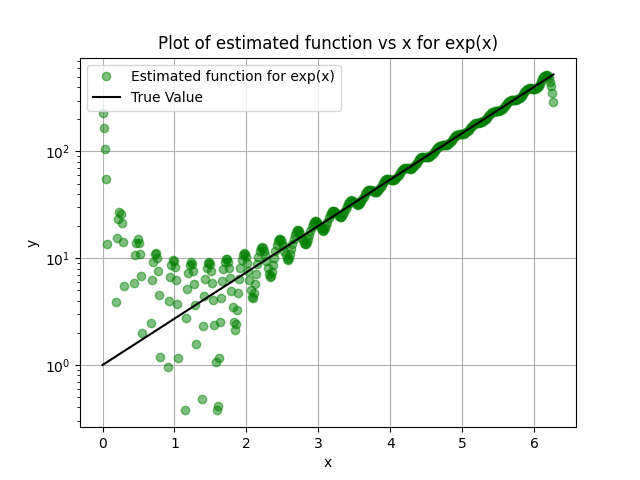
\includegraphics[scale=0.8]{Figure_13.png}
\end{figure}

\begin{figure}[H]
     \centering
     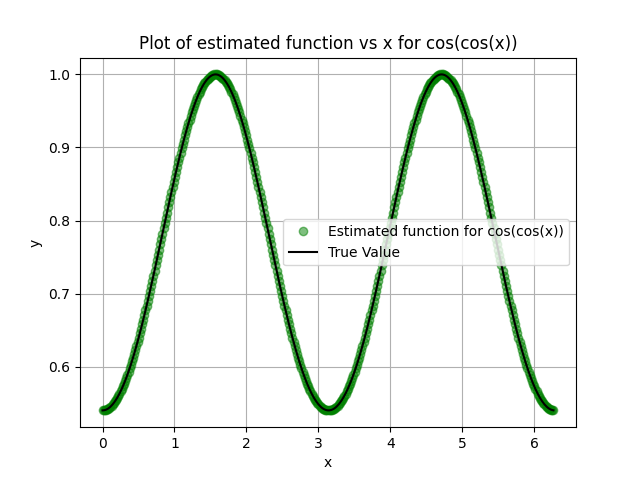
\includegraphics[scale=0.8]{Figure_14.png}
\end{figure}


We notice that the plot for $\cos(\cos(x))$ is almost exact, but the plot for $\exp(x)$ varies significantly near the edges. The reason is, as explained earlier, $\cos(\cos(x))$ is periodic, whereas $\exp(x)$ is aperiodic. Also, since the least squares approach is only approximate and $\exp(x)$ has a much higher gradient, this is expected. 


\section{Conclusion}
Thus, we have calculated the Fourier series coefficients in two different ways, one by direct integration and the other by least squares approximation. We notice that the least squares approach for the periodic function $\cos(\cos(x))$ is nearly exact, whereas this is not the case for aperiodic function $\exp(x)$. This is because of the high gradient characteristics of $\exp(x)$ and the periodic nature of $\cos(\cos(x))$.


\end{document}



 